\documentclass[aspectratio=169]{beamer}
\usepackage[utf8]{inputenc}
\usepackage[T1]{fontenc}
\usepackage{listings}

\usetheme{Madrid}
\usecolortheme{default}

%------------------------------------------------------------
\title[MapReduce]
{Hadoop MapReduce}

\author[Claudio, Gabriell]
{Claudio~Scheer\inst{1} \and Gabriell~Araujo\inst{1}}

\institute[PUCRS]
{
	\inst{1}
	Master's Degree in Computer Science\\
	Pontifical Catholic University of Rio Grande do Sul - PUCRS
}

\date[2020]
{High Performance for Big Data Applications}
%------------------------------------------------------------

%------------------------------------------------------------
\AtBeginSection[]
{
	\begin{frame}
		\frametitle{Table of Contents}

		\tableofcontents[currentsection]
	\end{frame}
}
%------------------------------------------------------------

\begin{document}

\frame{\titlepage}

%---------------------------------------------------------
\begin{frame}
	\frametitle{Table of Contents}

	\tableofcontents
\end{frame}
%---------------------------------------------------------

%---------------------------------------------------------
\section{Hadoop}

\begin{frame}
	\frametitle{What we mean by Hadoop}

	\begin{center}
		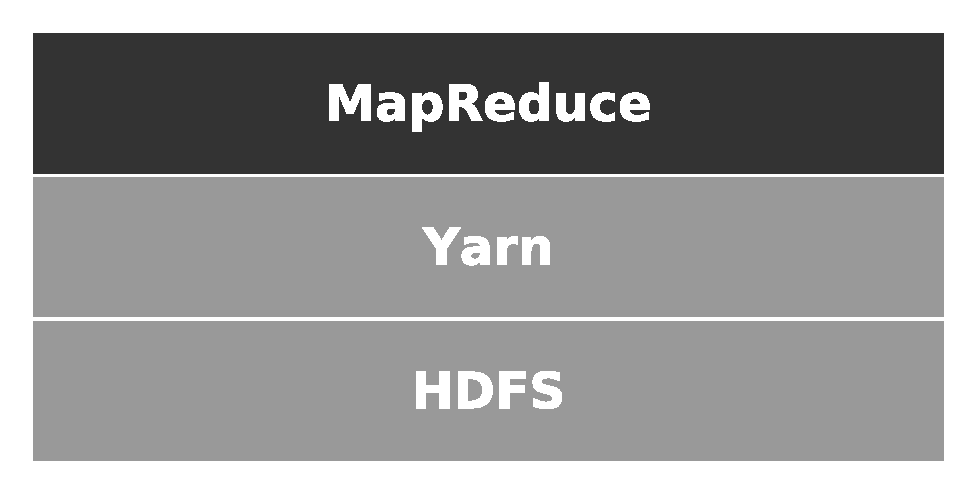
\includegraphics[height=1\textheight,width=0.6\textwidth,keepaspectratio]{./images/hadoop.pdf}
		{\tiny \href{https://data-flair.training/blogs/hadoop-ecosystem-components}{https://data-flair.training/blogs/hadoop-ecosystem-components}}
	\end{center}
\end{frame}

\begin{frame}
	\frametitle{MapReduce execution flow}

	\begin{center}
		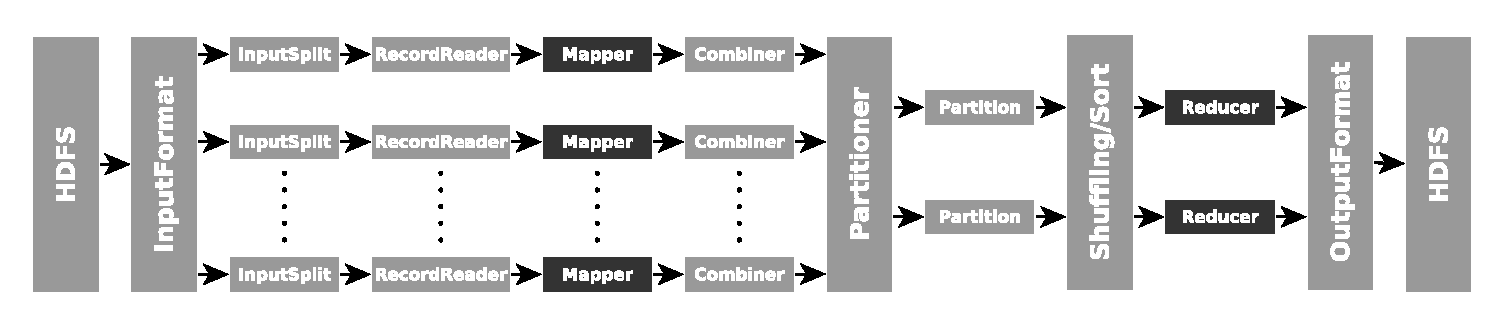
\includegraphics[height=1\textheight,width=1\textwidth,keepaspectratio]{./images/map-reduce.pdf}
		{\tiny \href{https://data-flair.training/blogs/hadoop-ecosystem-components}{https://data-flair.training/blogs/hadoop-ecosystem-components}}
	\end{center}
\end{frame}

\begin{frame}[fragile]
	\frametitle{Custom data types}

	\begin{columns}
		\column{0.4\textwidth}
		\begin{itemize}
			\item LongWritable = long;
			\item IntWritable = int;
			\item Text = String;
			\item \href{https://hadoop.apache.org/docs/current/api/org/apache/hadoop/io/package-summary.html}{Other data types (link);}
		\end{itemize}


		\column{0.6\textwidth}
		\begin{lstlisting}[language=java,basicstyle=\tiny,columns=fullflexible]
public class IntWritable implements WritableComparable<IntWritable> {
  private int value;

  public IntWritable(int value) { set(value); }

  public void set(int value) { this.value = value; }

  public int get() { return value; }

  @Override
  public void readFields(DataInput in) throws IOException {
    value = in.readInt();
  }

  @Override
  public void write(DataOutput out) throws IOException {
    out.writeInt(value);
  }

  @Override
  public int compareTo(IntWritable o) {
    int thisValue = this.value;
    int thatValue = o.value;
    return (thisValue < thatValue ? -1 : (thisValue == thatValue ? 0 : 1));
  }
}
        \end{lstlisting}
		{\tiny \href{https://github.com/apache/hadoop/blob/master/hadoop-common-project/hadoop-common/src/main/java/org/apache/hadoop/io/IntWritable.java}{\beamergotobutton{Source}}}
	\end{columns}
\end{frame}

\begin{frame}
	\frametitle{InputFormat}

	\begin{itemize}
		\item TextInputFormat: <LongWritable, Text>
		\item KeyValueTextInputFormat: <Text, Text>
		      \begin{itemize}
			      \item Key splitted by \textbackslash t;
		      \end{itemize}
		\item NLineInputFormat: <LongWritable, Text>
		      \begin{itemize}
			      \item {\scriptsize \texttt{config.setInt(NLineInputFormat.LINES\_PER\_MAP, 256)}};
		      \end{itemize}
		\item Custom InputFormat must implement \texttt{getSplits} and \texttt{getRecordReader};
	\end{itemize}

	\begin{center}
		{\tiny \href{https://hadoop.apache.org/docs/stable/api/org/apache/hadoop/mapred/InputFormat.html}{https://hadoop.apache.org/docs/stable/api/org/apache/hadoop/mapred/InputFormat.html}}
	\end{center}
\end{frame}

\begin{frame}
	\frametitle{InputSplit}

	\begin{itemize}
		\item Defines the level of parallelism;
		\item Splitted by the size of the block;
		      \begin{itemize}
			      \item 10TB/128MB = 82000
		      \end{itemize}
		\item It is a logical division of the input data;
	\end{itemize}

	\begin{center}
		{\tiny \href{https://hadoop.apache.org/docs/stable/hadoop-mapreduce-client/hadoop-mapreduce-client-core/MapReduceTutorial.html}{https://hadoop.apache.org/docs/stable/hadoop-mapreduce-client/hadoop-mapreduce-client-core/MapReduceTutorial.html}}
	\end{center}
\end{frame}

\begin{frame}[fragile]
	\frametitle{RecordReader}

	\begin{itemize}
		\item Split InputSplit into <key, value> pairs;
		      \begin{itemize}
			      \item Custom implementations can read values from outside the InputSplit;
		      \end{itemize}
		\item Lines greater than the max record length are ignored:
		      \begin{itemize}
			      \item {\scriptsize \texttt{config.setInt(LineRecordReader.MAX\_LINE\_LENGTH, Integer.MAX\_VALUE);}}
		      \end{itemize}
		\item Vanilla example:
		      \begin{lstlisting}[language=java,basicstyle=\tiny,columns=fullflexible]
        public void run(Context context) {
            setup(context);
            while (context.nextKeyValue()) {
                map(context.setCurrentKey(), context.getCurrentValue(), context);
            }
            cleanup(context);
        }
            \end{lstlisting}
	\end{itemize}
\end{frame}

\begin{frame}[fragile]
	\frametitle{Mapper}

	\begin{itemize}
		\item Maps <key1, value1> to <key2, value2>;
		\item Vanilla example:
		      \begin{lstlisting}[language=java,basicstyle=\tiny,columns=fullflexible]
        public class SimpleMapper extends Mapper<LongWritable, Text, Text, IntWritable> {
            private IntWritable one = new IntWritable(1);
            private Text word = new Text();

            @Override
            public void map(LongWritable key, Text value, Context context) {
                StringTokenizer itr = new StringTokenizer(value.toString());
                while (itr.hasMoreElements()) {
                    word.set(itr.nextToken());
                    context.write(word, one);
                }
            }
        }
            \end{lstlisting}
	\end{itemize}

	\begin{center}
		{\tiny \href{https://hadoop.apache.org/docs/current/hadoop-mapreduce-client/hadoop-mapreduce-client-core/MapReduceTutorial.html}{https://hadoop.apache.org/docs/current/hadoop-mapreduce-client/hadoop-mapreduce-client-core/MapReduceTutorial.html}}
	\end{center}
\end{frame}

\begin{frame}
	\frametitle{Combiner}

	\begin{itemize}
		\item Reduces data transfer between mapper and reducer;
		\item Reduces the amount of data to be processed in the reducer;
	\end{itemize}

	\begin{center}
		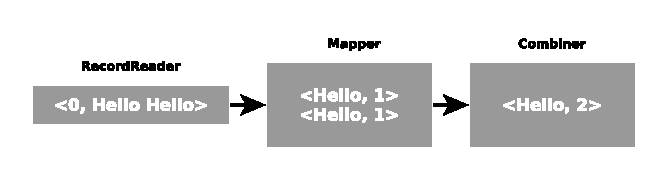
\includegraphics[height=1\textheight,width=0.8\textwidth,keepaspectratio]{./images/combiner.pdf}
	\end{center}
\end{frame}

\begin{frame}[fragile]
	\frametitle{Partitioner}

	\begin{itemize}
		\item Redirects the Combiner output to a specific reducer;
		\item Has the same number as the number of reducers;
		\item Used only when there is more than one reducer;
		\item Vanilla example:
		      \begin{lstlisting}[language=java,basicstyle=\tiny,columns=fullflexible]
        public class StupidPartitioner extends Partitioner<Text, IntWritable> {
            public int getPartition(Text key, IntWritable value, int numPartitions) {
                if (value.get() < 35) {
                    return 0;
                } else {
                    return 1;
                }
            }
        }
            \end{lstlisting}
	\end{itemize}

	\begin{center}
		{\tiny \href{https://hadoop.apache.org/docs/stable/api/org/apache/hadoop/mapreduce/Partitioner.html}{https://hadoop.apache.org/docs/stable/api/org/apache/hadoop/mapreduce/Partitioner.html}}
	\end{center}
\end{frame}

\begin{frame}
	\frametitle{Shuffle/Sort}

	\begin{itemize}
		\item Collects output from the mappers to the reducers using HTTP requests;
		\item Sorts the collected <key, value> pairs based on the key;
		      \begin{itemize}
			      \item \texttt{job.setSortComparatorClass(StupidSortComparator.class);}
		      \end{itemize}
	\end{itemize}

	\begin{center}
		{\tiny \href{https://hadoop.apache.org/docs/stable/hadoop-mapreduce-client/hadoop-mapreduce-client-core/PluggableShuffleAndPluggableSort.html}{https://hadoop.apache.org/docs/stable/hadoop-mapreduce-client/hadoop-mapreduce-client-core/PluggableShuffleAndPluggableSort.html}}
		{\tiny \href{https://hadoop.apache.org/docs/stable/hadoop-mapreduce-client/hadoop-mapreduce-client-core/EncryptedShuffle.html}{https://hadoop.apache.org/docs/stable/hadoop-mapreduce-client/hadoop-mapreduce-client-core/EncryptedShuffle.html}}
	\end{center}
\end{frame}

\begin{frame}[fragile]
	\frametitle{Reducer}

	\begin{itemize}
		\item Reduces <key2, list(value2)> to <key3, value3>;
		\item Change the number of reducers:
		      \begin{itemize}
			      \item \texttt{job.setNumReduceTasks(2);}
		      \end{itemize}
		\item Vanilla example:
		      \begin{lstlisting}[language=java,basicstyle=\tiny,columns=fullflexible]
        public static class SimpleReducer extends Reducer<Text, IntWritable, Text, IntWritable> {
            private IntWritable result = new IntWritable();

            @Override
            public void reduce(Text key, Iterable<IntWritable> values, Context context) {
                int sum = 0;
                for (IntWritable val : values) {
                    sum += val.get();
                }
                result.set(sum);
                context.write(key, result);
            }
        }
            \end{lstlisting}
	\end{itemize}

	\begin{center}
		{\tiny \href{https://hadoop.apache.org/docs/current/hadoop-mapreduce-client/hadoop-mapreduce-client-core/MapReduceTutorial.html}{https://hadoop.apache.org/docs/current/hadoop-mapreduce-client/hadoop-mapreduce-client-core/MapReduceTutorial.html}}
		{\tiny \href{https://docs.cloudera.com/HDPDocuments/HDP2/HDP-2.6.5/bk_command-line-installation/content/determine-hdp-memory-config.html}{https://docs.cloudera.com/HDPDocuments/HDP2/HDP-2.6.5/bk\_command-line-installation/content/determine-hdp-memory-config.html}}
	\end{center}
\end{frame}

\begin{frame}
	\frametitle{OutputFormat}

	\begin{itemize}
		\item Specifies how reducer output will be written;
		      \begin{itemize}
			      \item {\scriptsize \texttt{config.set(TextOutputFormat.SEPARATOR, ``,'');}}
		      \end{itemize}
		\item Allows to write multiple outputs;
		      \begin{itemize}
			      \item {\tiny \href{https://hadoop.apache.org/docs/stable/api/org/apache/hadoop/mapred/lib/MultipleOutputs.html}{https://hadoop.apache.org/docs/stable/api/org/apache/hadoop/mapred/lib/MultipleOutputs.html}}
		      \end{itemize}
	\end{itemize}
\end{frame}
%---------------------------------------------------------

%---------------------------------------------------------
\section{General}

\begin{frame}
	\frametitle{How many maps?}

	\begin{itemize}
		\item Usually defined by the size of the input;
		\item Around 10-100 maps per-node;
	\end{itemize}
\end{frame}

\begin{frame}
	\frametitle{How many reducers?}

	\begin{itemize}
		\item 0.95 or 1.75 multiplied by (<number of nodes> * <number of maximum containers per node>);
		      \begin{itemize}
			      \item 1.75 has a much better load balancing;
			      \item Scale factor are not using whole numbers to reserve a few slots for speculative-tasks and failed tasks;
		      \end{itemize}
	\end{itemize}

	\begin{center}
		{\tiny \href{https://docs.cloudera.com/HDPDocuments/HDP2/HDP-2.6.5/bk_command-line-installation/content/determine-hdp-memory-config.html}{https://docs.cloudera.com/HDPDocuments/HDP2/HDP-2.6.5/bk\_command-line-installation/content/determine-hdp-memory-config.html}}
	\end{center}
\end{frame}

\begin{frame}
	\frametitle{Counters}

	\begin{itemize}
	    \item Monitors specific action in the mapreduce job;
		\item User can define custom counters;
	\end{itemize}
\end{frame}

\begin{frame}
	\frametitle{Uber task}

	\begin{itemize}
	    \item Used when the cost of negotiating a container on a remote node is more than running the task on the JVM Application Master itself;
		\item Changing default values in \texttt{mapred-site.xml}:
		      \begin{itemize}
			      \item \texttt{mapreduce.job.ubertask.enable}
			      \item \texttt{mapreduce.job.ubertask.maxmaps}
			      \item \texttt{mapreduce.job.ubertask.maxreduces}
			      \item \texttt{mapreduce.job.ubertask.maxbytes}
		      \end{itemize}
	\end{itemize}
\end{frame}

\begin{frame}
	\frametitle{Other settings}

	\begin{itemize}
		\item Useful settings that can be changed in \texttt{mapred-site.xml}:
		      \begin{itemize}
			      \item \texttt{mapreduce.job.running.map.limit}: The maximum number of simultaneous map tasks per job;
			      \item \texttt{mapreduce.job.max.map}: Limit on the number of map tasks allowed per job;
			      \item \texttt{mapreduce.input.fileinputformat.split.maxsize}: Default split size;
		      \end{itemize}
	\end{itemize}
\end{frame}
%---------------------------------------------------------

%---------------------------------------------------------
\section{Examples}

\begin{frame}
	\frametitle{Unquestionable!}

	\begin{center}
		
\includegraphics[height=1\textheight,width=0.5\textwidth,keepaspectratio]{./images/show-me-the-code.jpg}
	\end{center}
\end{frame}

\begin{frame}
	\frametitle{Objectives}
	
	\begin{itemize}
	    \item How to setup Hadoop on a multi-node cluster;
	    \item Show coding examples;
		\item Show how to monitor running jobs;
	\end{itemize}
\end{frame}

\begin{frame}
    \frametitle{That's all Folks!}

	\begin{itemize}
	    \item \href{https://github.com/claudioscheer/hadoop-hello-world}{hadoop-hello-world};
	    \item \href{https://github.com/claudioscheer/claudioscheer.github.io/blob/master/posts/hadoop/install-hadoop-multi-node-cluster.md}{Install Hadoop in a multi-node cluster scenario};
	    \item \href{https://github.com/claudioscheer/claudioscheer.github.io/blob/master/posts/hadoop/useful-things-about-hadoop.md}{Useful things about Hadoop};
	\end{itemize}
\end{frame}
%---------------------------------------------------------

\end{document}
